% Beyond Density Matrices: Geometric Quantum States
% 	formerly:
% What is a Quantum State?
%
% fa: 4/31/20, 5/4/20, 7/15/20
% jpc: 5/1/20, 5/6/20, 7/19/20

%\documentclass[draft,nofootinbib,prl,twocolumn,showpacs,showkeys,groupaddress,preprintnumbers,floatfix]{revtex4-1}
\documentclass[draft,nofootinbib,pre,twocolumn,showpacs,showkeys,preprintnumbers,floatfix]{revtex4-1}

\usepackage{dynlearn}
\usepackage{physics}
\usepackage{multibib}
\newcites{SM}{SM References}
% \usepackage[utf8]{inputenc}
\usepackage{mathrsfs}
\usepackage[english]{babel}
\usepackage{amssymb,amscd}
\newtheorem{theorem}{Theorem}
\newtheorem{hypothesis}{Hypothesis}

% \newcommand{\norm}[1]{\left\Vert#1\right\Vert}
% \newcommand{\abs}[1]{\left\vert#1\right\vert}
% \newcommand{\set}[1]{\left\{#1\right\}}
% \newcommand{\R}{\mathbb{R}}
\newcommand{\e}{\mathrm{e}}
\newcommand{\Hilb}{\mathcal{H}}
\newcommand{\eps}{\varepsilon}
\newcommand{\To}{\longrightarrow}
\newcommand{\BX}{\mathbf{B}(X)}
\newcommand{\A}{\mathcal{A}}
\newcommand{\HH}{\Hilb}
\newcommand{\g}{\mathfrak{g}}
\newcommand{\Ug}{\mathcal{U}\mathfrak{g}}
\newcommand{\Tg}{\mathcal{T}\mathfrak{g}}
\newcommand{\Sg}{\mathcal{S}\mathfrak{g}}
\newcommand{\Us}{\mathcal{U}\mathfrak{s}}
\newcommand{\Ss}{\mathcal{S}\mathfrak{s}}
% \DeclareMathOperator{\Tr}{Tr}
\DeclareMathOperator*{\argmax}{arg\,max}
\DeclareMathOperator*{\argmin}{arg\,min}
\newcommand{\Ut}[1]{\undertilde{#1}}
\newcommand{\1}{\mathbbm{1}}
\newcommand{\circled}[1]{\tikz[baseline=(C.base)]\node[draw,circle,inner sep=1. 2pt,line width=0.2mm,](C) {\small #1};\!}
\newcommand{\Pexp}[1]{\mathrm{Pexp} \left[ #1 \right] }
\newcommand{\Ch}[1]{ \mathrm{Ch} \; #1}
\newcommand{\Sh}[1]{ \mathrm{Sh} \; #1}
% \newcommand{\Ket}[1]{ \left| #1 \right\rangle}
% \newcommand{\Bra}[1]{ \left\langle #1 \right|}
\newcommand{\Scal}[2]{ \left\langle #1 | #2 \right\rangle}
\newcommand{\KetQ}[1]{ \left| #1 \right]}
\newcommand{\BraQ}[1]{ \left[ #1 \right|}
\newcommand{\ScalQ}[2]{ \left[ #1 | #2 \right]}
\newcommand{\Miss}[2]{ \left[ #1 | #2 \right\rangle}
\newcommand{\MissQ}[2]{ \left\langle #1 | #2 \right]}
\newcommand{\ZT}{\undertilde{z}}
\newcommand{\Z}{\zeta}
\newcommand{\MV}[1]{\left\langle #1 \right\rangle}
\newcommand{\MC}[1]{\left\langle #1 \right\rangle_{\mathrm{mc}}}
% \newcommand{\braket}[2]{\langle #1 | #2 \rangle}
% \newcommand{\ketbra}[2]{| #2 \rangle\langle #1 |}
% \newcommand{\ket}[1]{| #1 \rangle}
% \newcommand{\bra}[1]{\langle #1 |}
\renewcommand{\equiv}{\coloneqq}
\newcommand{\PP}[4]{\mathbin{_{#2} P^{#1}_{#3}} \left[ #4 \right]}
\newcommand{\intP}{\int_{\mathcal{P}(\mathcal{H})} \!\!\!\!\!\!\!\!\!}
\newcommand{\intPB}{\int_{\mathcal{P}(\overline{\mathcal{H}})} \!\!\!\!\!\!\!\! \!}
\newcommand{\PH}{\mathcal{P}(\mathcal{H})}

\def\d{\delta}
\def\f{\frac}
\def\om{\omega}
\def\w{\wedge}
\def\la{\langle}
\def\ra{\rangle}
\newcommand{\p}{\partial}
\newcommand{\n}{\nabla}

\newcommand{\cg}[1]{{\color{blue}[[CG: #1]]}}
\newcommand{\fa}[1]{{\color{red}[[FA: #1]]}}
\newcommand{\cut}[1]{{\color{purple}[[CUT?: #1]]}}

\newenvironment{entry}
  {\begin{list}{--}{
      \setlength{\topsep}{0pt}
      \setlength{\itemsep}{0pt}
      \setlength{\parsep}{0pt}
      \setlength{\labelwidth}{5pt}
      \setlength{\itemindent}{0pt}}}{\end{list}}

\def\tbf #1 {\textbf{#1} }

\begin{document}

\def\ourTitle{%
% Interpretation of the Geometric Quantum State
% What is a Quantum State?
A kinetic theory of quantum information
}

\def\ourAbstract{%
TBD
}

\def\ourKeywords{%
Quantum Mechanics, Geometric Quantum Mechanics
}

\hypersetup{
  pdfauthor={Fabio Anza},
  pdftitle={\ourTitle},
  pdfsubject={\ourAbstract},
  pdfkeywords={\ourKeywords},
  pdfproducer={},
  pdfcreator={}
}

%%%%%%%%%%%%%%%%%%%%%%%%%%%%%%%%%%%%%%%%%%%%%%%%%%%%%%%%%%%%%%%%%%%%%%%%%%%%%%%

\title{\ourTitle}

\author{Fabio Anza}
\email{fanza@ucdavis.edu}

%\author{James P. Crutchfield}
%\email{chaos@ucdavis.edu}

\affiliation{Complexity Sciences Center and Physics Department,
University of California at Davis, One Shields Avenue, Davis, CA 95616}

\date{\today}
\bibliographystyle{unsrt}

\begin{abstract}
\ourAbstract
\end{abstract}

\keywords{\ourKeywords}

\pacs{
05.45.-a  %  Nonlinear dynamics and nonlinear dynamical systems
89.75.Kd  %  Complex Systems: Patterns
89.70.+c  %  Information science
05.45.Tp  %  Time series analysis
%02.50.Ey  %  Stochastic processes
%02.50.-r  %  Probability theory, stochastic processes, and statistics
%02.50.Ga  %  Markov processes
%%%%%%%FROM HERE%%%%%%
%05.20.-y  %  Classical statistical mechanics
%02.40.−k %Geometry, differential geometry, and topology
%03.65.−w %Quantum mechanics
%03.67.−a %Quantum information
%05.30.−d %Quantum statistical mechanics
%05.70.−a %Thermodynamics
%%%%%%%TO HERE%%%%%%
}

\preprint{\arxiv{2008.08682}}

\date{\today}
\maketitle

% \tableofcontents

% \setstretch{1.1}

% Collides with table of contents formatting
% \listoffixmes

% {\bf Lead Paragraph:
% }

\section*{Introduction.} The study of transport phenomena is crucial to harness 
the dynamical properties of natural systems. In this sense, transport theories are 
phenomenological descriptions of the nonequilibrium behavior of a system. Well-known 
examples are the theories of transport of charge, mass and heat. Most of them, were 
originally formulated to understand macroscopic phenomena like (in the case of 
mass transport) the tendency of a system to transfer mass in order to minimise the 
concentration difference. Over time, they were put on more rigorous ground using 
statistical mechanics and kinetic theory. Most notably, Boltzmann used this approach
to describe the behavior of gases, and explain the rise of macroscopic irreversibility from 
the underlying time-symmetric classical mechanics. After Boltzmann's work, the core idea 
of treating motion and interaction in a statistical way has led to innumerable advances, both 
of fundamental and applied nature. With the rise of quantum theory, these techniques have 
also been adapted to include quantum fluctuations, leading to improved descriptions of 
transport phenomena at the nanoscale.
While nowadays the use of kinetic and transport theories is ubiquitous, these techniques
have not been leveraged to study quantum information in closed and open quantum systems. 
Thus, in this work, we attempt to lay a bridge between the field of quantum information and 
that of transport theories. We do so by building a kinetic theory of quantum information for 
closed and open quantum systems. The main goal of this work is to provide a consistent definition
for common tools such as fluxes and sink/sources which 

At the technical level, this is done by leveraging recent work \cite{Anza2020a,Anza2020b} on 
Geometric Quantum Mechanics: a differential-geometric approach to quantum mechanics that 
gets rid of the phase redundancy of the Hilbert space. The geometric formalism maps the Hilbert 
space onto a space of pure states that has the structure of a classical phase-space, with 
canonically conjugated coordinates.

The paper is organized as follows. In Section \ref{sec:GQM} we give a brief summary of 
GQM, and of the tools introduced in \cite{Anza2020a,Anza2020b}, both of which are needed.
In Section \ref{sec:IT} we give the first result: a microscopic derivation of the continuity equation 
for the information transport in quantum systems, with appropriate, microscopic definitions for 
phenomenological quantities such as fluxes and sink/sources terms. In Section \ref{sec:DYN}
we give the second result: a general equation of motion for the probability distribution that an open
quantum system is found in one of its quantum states. In Section \ref{sec:EXAMPLES} we provide
a few concrete examples, supported by numerical analysis. Eventually, in Section \ref{sec:FINAL}
we provide a quick summary and draw some conclusions.
 


%In the last fifty years we have witnessed an increasing use of
%information-theoretic techniques in virtually all scientific disciplines. Among all of them, the 
%cross-fertilization between physics and information theory has proven to be particularly fruitful.
%Within physics itself, it is hard to overstate the rise of quantum computing and quantum information 
%theory which, together with the modern experimental means to control nanoscale systems at the 
%level of individual components, has been addressed as a second quantum revolution \cite{Dow03}, 
%whose goal is to bring forth a new set of \emph{quantum technologies}. 
%While much work has been done to better understand the physical nature of information, when 
%compared to other fundamental concepts, such as the concept of energy, it is opinion of the author
%that our understanding is still very much at the 


%Within this larger perspective, in this work we address a single question: can we talk about information
%as a localized quantity, which moves around and can be exchanged?




\section{Geometric Quantum Mechanics}
\label{sec:GQM}
References
\cite{STROCCHI1966,Miel68,Kibble1979,Heslot1985,Page87,And90,Gibbons1992,Ashtekar1995,Ashtekar1999,Brody2001,Bengtsson2017,Carinena2007,Chruscinski2006,Marmo2010,Avron2020,Pastorello2015,Pastorello2015a,Pastorello2016,Clemente-Gallardo2013}
give a comprehensive introduction to GQM. Here, we briefly summarize only the
elements we need, working with Hilbert spaces $\mathcal{H}$ of finite dimension $D$.

Pure states are points in the complex projective manifold $\mathcal{P}\left(
\mathcal{H} \right)=\mathbb{C}\mathrm{P}^{D-1}$. Therefore, given an arbitrary
basis $\left\{\ket{e_\alpha} \right\}_{\alpha=0}^{D-1}$, a pure state is
parametrized by $D$ complex homogeneous coordinates $Z = \left\{      Z^\alpha\right\}$, up to
normalization and an overall phase:
\begin{align*}
\ket{\psi} = \sum_{\alpha=0}^{D-1} Z^\alpha \ket{e_\alpha}
  ~,
\end{align*}
where $Z \in \mathbb{C}^{D}$, $Z \sim \lambda Z$, and $\lambda \in
\mathbb{C}/\left\{ 0\right\}$. If the system consists of a single qubit, for
example, one can always use probability-phase coordinates $Z = (\sqrt{1-p},\sqrt{p} e^{i\nu})$.

An \emph{observable} is a function $\mathcal{O}(Z) \in
\mathbb{R}$ that associates to each point  $Z \in \mathcal{P}(\mathcal{H})$ the
expectation value $\bra{\psi} \mathcal{O} \ket{\psi}/\braket{\psi}{\psi}$ of the corresponding
operator $\mathcal{O}$ on state $\ket{\psi}$ with coordinates $Z$:
\begin{align}
\mathcal{O}(Z) = \frac{\sum_{\alpha,\beta} \mathcal{O}_{\alpha,\beta}Z^\alpha \overline{Z}^\beta}{\sum_{\gamma} \left\vert Z^\gamma\right\vert^2}
  ~,
\label{eq:GQM_Observable}
\end{align}
where $\mathcal{O}_{\alpha \beta}$ is Hermitian $\mathcal{O}_{\beta,\alpha} = \overline{\mathcal{O}}_{\alpha,\beta}$.

Measurement outcome probabilities are determined by \emph{positive
operator-valued measurements} (POVMs) $\left\{E_j\right\}_{j=1}^n$ applied to a
state \cite{Nielsen2010,Heinosaari2012}. They are nonnegative operators
$E_j\geq 0$, called \emph{effects}, that sum up to the identity: $\sum_{j=1}^n
E_j = \mathbb{I}$. In GQM they consist of nonnegative real functions $E_j(Z)\ge
0$ on $\mathcal{P}(\mathcal{H})$ whose sum is always unity:
\begin{align}
E_j(Z) = \frac{\sum_{\alpha,\beta}
  \left(E_j\right)_{\alpha,\beta} Z^\alpha \overline{Z}^\beta}{\sum_{\gamma} \left\vert Z^\gamma \right\vert^2}
  ~,
\label{eq:GQM_POVMs}
\end{align}
where $\sum_{j=1}^{n}E_j(Z) = 1$.

The projective Hilbert space of the pure states of a quantum system $\mathcal{P}(\mathcal{H})$ has a preferred
metric $g_{FS}$---the \emph{Fubini-Study metric} \cite{Bengtsson2017}---and an
associated volume element $dV_{FS}$ that is coordinate-independent and
invariant under unitary transformations. The geometric derivation of $dV_{FS}$
is beyond our immediate goals here. That said, it is sufficient to give its
explicit form in the probability-phase coordinate system $Z^{\alpha} =
\sqrt{p_\alpha}e^{i\nu_\alpha}$ that we use for explicit calculations: 
\begin{align*}
dV_{FS}
  & = \sqrt{\det g_{FS}}
  \prod_{\alpha=0}^{D-1} dZ^\alpha d\overline{Z}^\alpha \\
  & =  \prod_{\alpha=1}^{D-1} \frac{dp_\alpha d\nu_\alpha}{2}
  ~.
\end{align*}
Notice how $p_0$ and $\nu_0$ are not involved. This is due to
$\mathcal{P}(\mathcal{H})$'s projective nature which guarantees that we can
choose a coordinate patch in which $p_0 = 1 - \sum_{\alpha=1}^{D-1}p_\alpha$
and $\nu_0 = 0$.

\paragraph*{Geometric quantum states.}
This framework makes it very natural to view a quantum state as a functional
encoding that associates expectation values to observables, paralleling the
$C^{*}$-algebra formulation of quantum mechanics \cite{Strocchi2008a}. 
The idea is that one considers probability density functions on $\mathcal{P}(\mathcal{H})$ (as $q(Z)$),
together with observable functions (as $\mathcal{O}(Z)$). This was introduced 
in Ref. \cite{Brody2001} and here we give a quick summary.

States are functionals $P[\mathcal{O}]$ from the algebra of
observables $\mathcal{A}$ to the real line: 
\begin{align}
P_q[\mathcal{O}]
  = \int_{\mathcal{P}(\mathcal{H})} q(Z) \mathcal{O}(Z) dV_{FS}
  ~,
\label{eq:gqs}
\end{align}
where $\mathcal{O} \in \mathcal{A}$, $q(Z) \geq 0$ is the
normalized distribution associated with functional $P$:
\begin{align*}
P_q[\mathbb{I}] = \int_{\mathcal{P}(\mathcal{H})}
  q(Z) dV_{FS}  = 1
  ~,
\end{align*}
and $P_q[\mathcal{O}] \in \mathbb{R}$. 
In this way, pure states $\ket{\psi_0}$ are functionals with a Dirac-delta
distribution $p_0(Z) = \widetilde{\delta}\left[ Z - Z_0\right]$:
\begin{align*}
P_{0}[\mathcal{O}] &= \intP \widetilde{\delta}(Z-Z_0)\mathcal{O}(Z) dV_{FS} \\
  & = \mathcal{O}(Z_0)  = \bra{\psi_0}\mathcal{O}\ket{\psi_0}
  ~.
\end{align*}
$\widetilde{\delta}(Z-Z_0)$ is shorthand for a coordinate-covariant Dirac-delta in
arbitrary coordinates. In homogeneous coordinates this reads:
\begin{align*}
\widetilde{\delta}(Z - Z_0) \coloneqq \frac{1}{\sqrt{\det g_{FS}}}
  \prod_{\alpha=0}^{D-1} \delta(X^\alpha - X^\alpha_0)
  \delta(Y^\alpha - Y^\alpha_0)
  ~,
\end{align*}
where $Z^\alpha = X^\alpha + iY^\alpha$. In $(p_\alpha,\nu_\alpha)$ coordinates
this becomes simply:
\begin{align*}
\widetilde{\delta}(Z - Z_0) = \prod_{\alpha=1}^{D-1} 2\delta(p_\alpha - p_\alpha^0) \delta(\nu_\alpha - \nu_\alpha^0)
  ~,
\end{align*}
where the coordinate-invariant nature of the functionals $P_q[\mathcal{O}]$ is
now apparent.

In this way, too, mixed states:
\begin{align*}
\rho = \sum_{j}\lambda_j \ket{\lambda_j}\bra{\lambda_j}
\end{align*}
are convex combinations of these Dirac-delta functionals:
\begin{align*}
q_{\mathrm{mix}}(Z) = \sum_{j}\lambda_j \widetilde{\delta}(Z-Z_j)
  ~. 
\end{align*}
Thus, expressed as functionals from observables to the real line, mixed states
are:
\begin{align}
P_{\mathrm{mix}}\left[ \mathcal{O}\right]
  & = \sum_{j} \lambda_j \bra{\lambda_j}\mathcal{O}\ket{\lambda_j}
  ~.
\label{eq:Functional}
\end{align}

Equipped with this tools, one identifies the distribution $q(Z)$ of Eq.
(\ref{eq:gqs}) as a system's \emph{geometric quantum state}. This is a
generalized notion of quantum state.

A simple example of a geometric quantum state is the 
\emph{geometric canonical ensemble}:
\begin{align*}
q(Z) = \frac{1}{Q_\beta} e^{-\beta h(Z)}
  ~,
\end{align*}
where:
\begin{align*}
  Q_\beta & = \int dV_{FS} e^{-\beta h(Z)} ~, \\
  h(Z) & = \bra{\psi(Z)}H\ket{\psi(Z)} ~,
\end{align*}
and $H$ is the system's Hamiltonian operator. This was introduced in 
Refs. \cite{Brody1998}. References \cite{Brody2016} and \cite{Anza20b} 
investigated its potential role in establishing a quantum foundation of
thermodynamics that is an alternative to that based on Gibbs ensembles and von
Neumann entropy. 

\paragraph*{Density matrix.}
The connection between geometric quantum states and density matrices is
two-fold. On the one hand, when $q(Z)$ falls into one of the
two aforementioned cases---Dirac-deltas or finite convex combinations of
them---the present formalism is equivalent to the standard one. However, not
all functionals fall into the Dirac-delta form. Given this, $q(Z)$ is clearly a
more general notion of a quantum system's state than density matrices.

On the other hand, given an arbitrary $q(Z)$, there is a unique
density matrix $\rho^{q}$ associated to $q$:
\begin{align}
\rho^q_{\alpha \beta} & = P_q[Z^\alpha \overline{Z}^\beta] \nonumber \\
  & = \intP dV_{FS} \, q(Z)  \, Z^\alpha \overline{Z}^\beta
  ~.
\label{eq:densitymatrix}
\end{align}
Owing to the specific form of POVMs on $\mathcal{P}(\mathcal{H})$, recall Eq. (\ref{eq:GQM_POVMs}), they
are sensitive to $q(Z)$ only via $\rho^q$. Therefore, if two geometric quantum states 
$q_1$ and $q_2$ induce the same density matrix $\rho^{q_1} = \rho^{q_2}$, then all POVMs
produce the same outcomes.

A well-known consequence of this fact is that two density matrices with the
same barycenter are considered equal, even if they describe experiments with
different physical configurations. In these cases, the statistics of POVM
outcomes are described by the same density matrix. Note that this statement
does not mean that the two physical configurations are the same. Rather, it
means that there is no POVM on the system that distinguishes between $q_1$ and
$q_2$.

To emphasize, consider the example of two geometric quantum states, $q_1$ and
$q_2$, with very different characteristics:
\begin{align*}
q_1(Z) & = 0.864~\tilde{\delta}(Z - Z_{+}) + 0.136~\tilde{\delta}(Z - Z_{-})~,\\
q_2(Z) & = \frac{1}{Q} e^{-\frac{1}{2} \overline{Z}\rho^{-1}Z } 
  ~,
\end{align*}
where $Q = \int_{\mathbb{C}P^1} dV_{FS} e^{-\frac{1}{2}Z \rho^{-1}
\overline{Z}}$, $Z_+ = (0.657,0.418 + i 0.627)$, and $Z_- =
(0.754,-0.364-i0.546)$. However, states $q_1$ and $q_2$ have same density
matrix $\rho$ ($\rho_{00} = 0.45 = 1- \rho_{11}$ and $\rho_{01} = 0.2 - i 0.3
= \rho_{10}^{*}$) and so the same POVM outcomes. From Fig. \ref{fig:Example}
one appreciates the profound difference between $q_1$ and $q_2$, despite the
equality of their POVM statistics.

\begin{figure}[h]
\centering
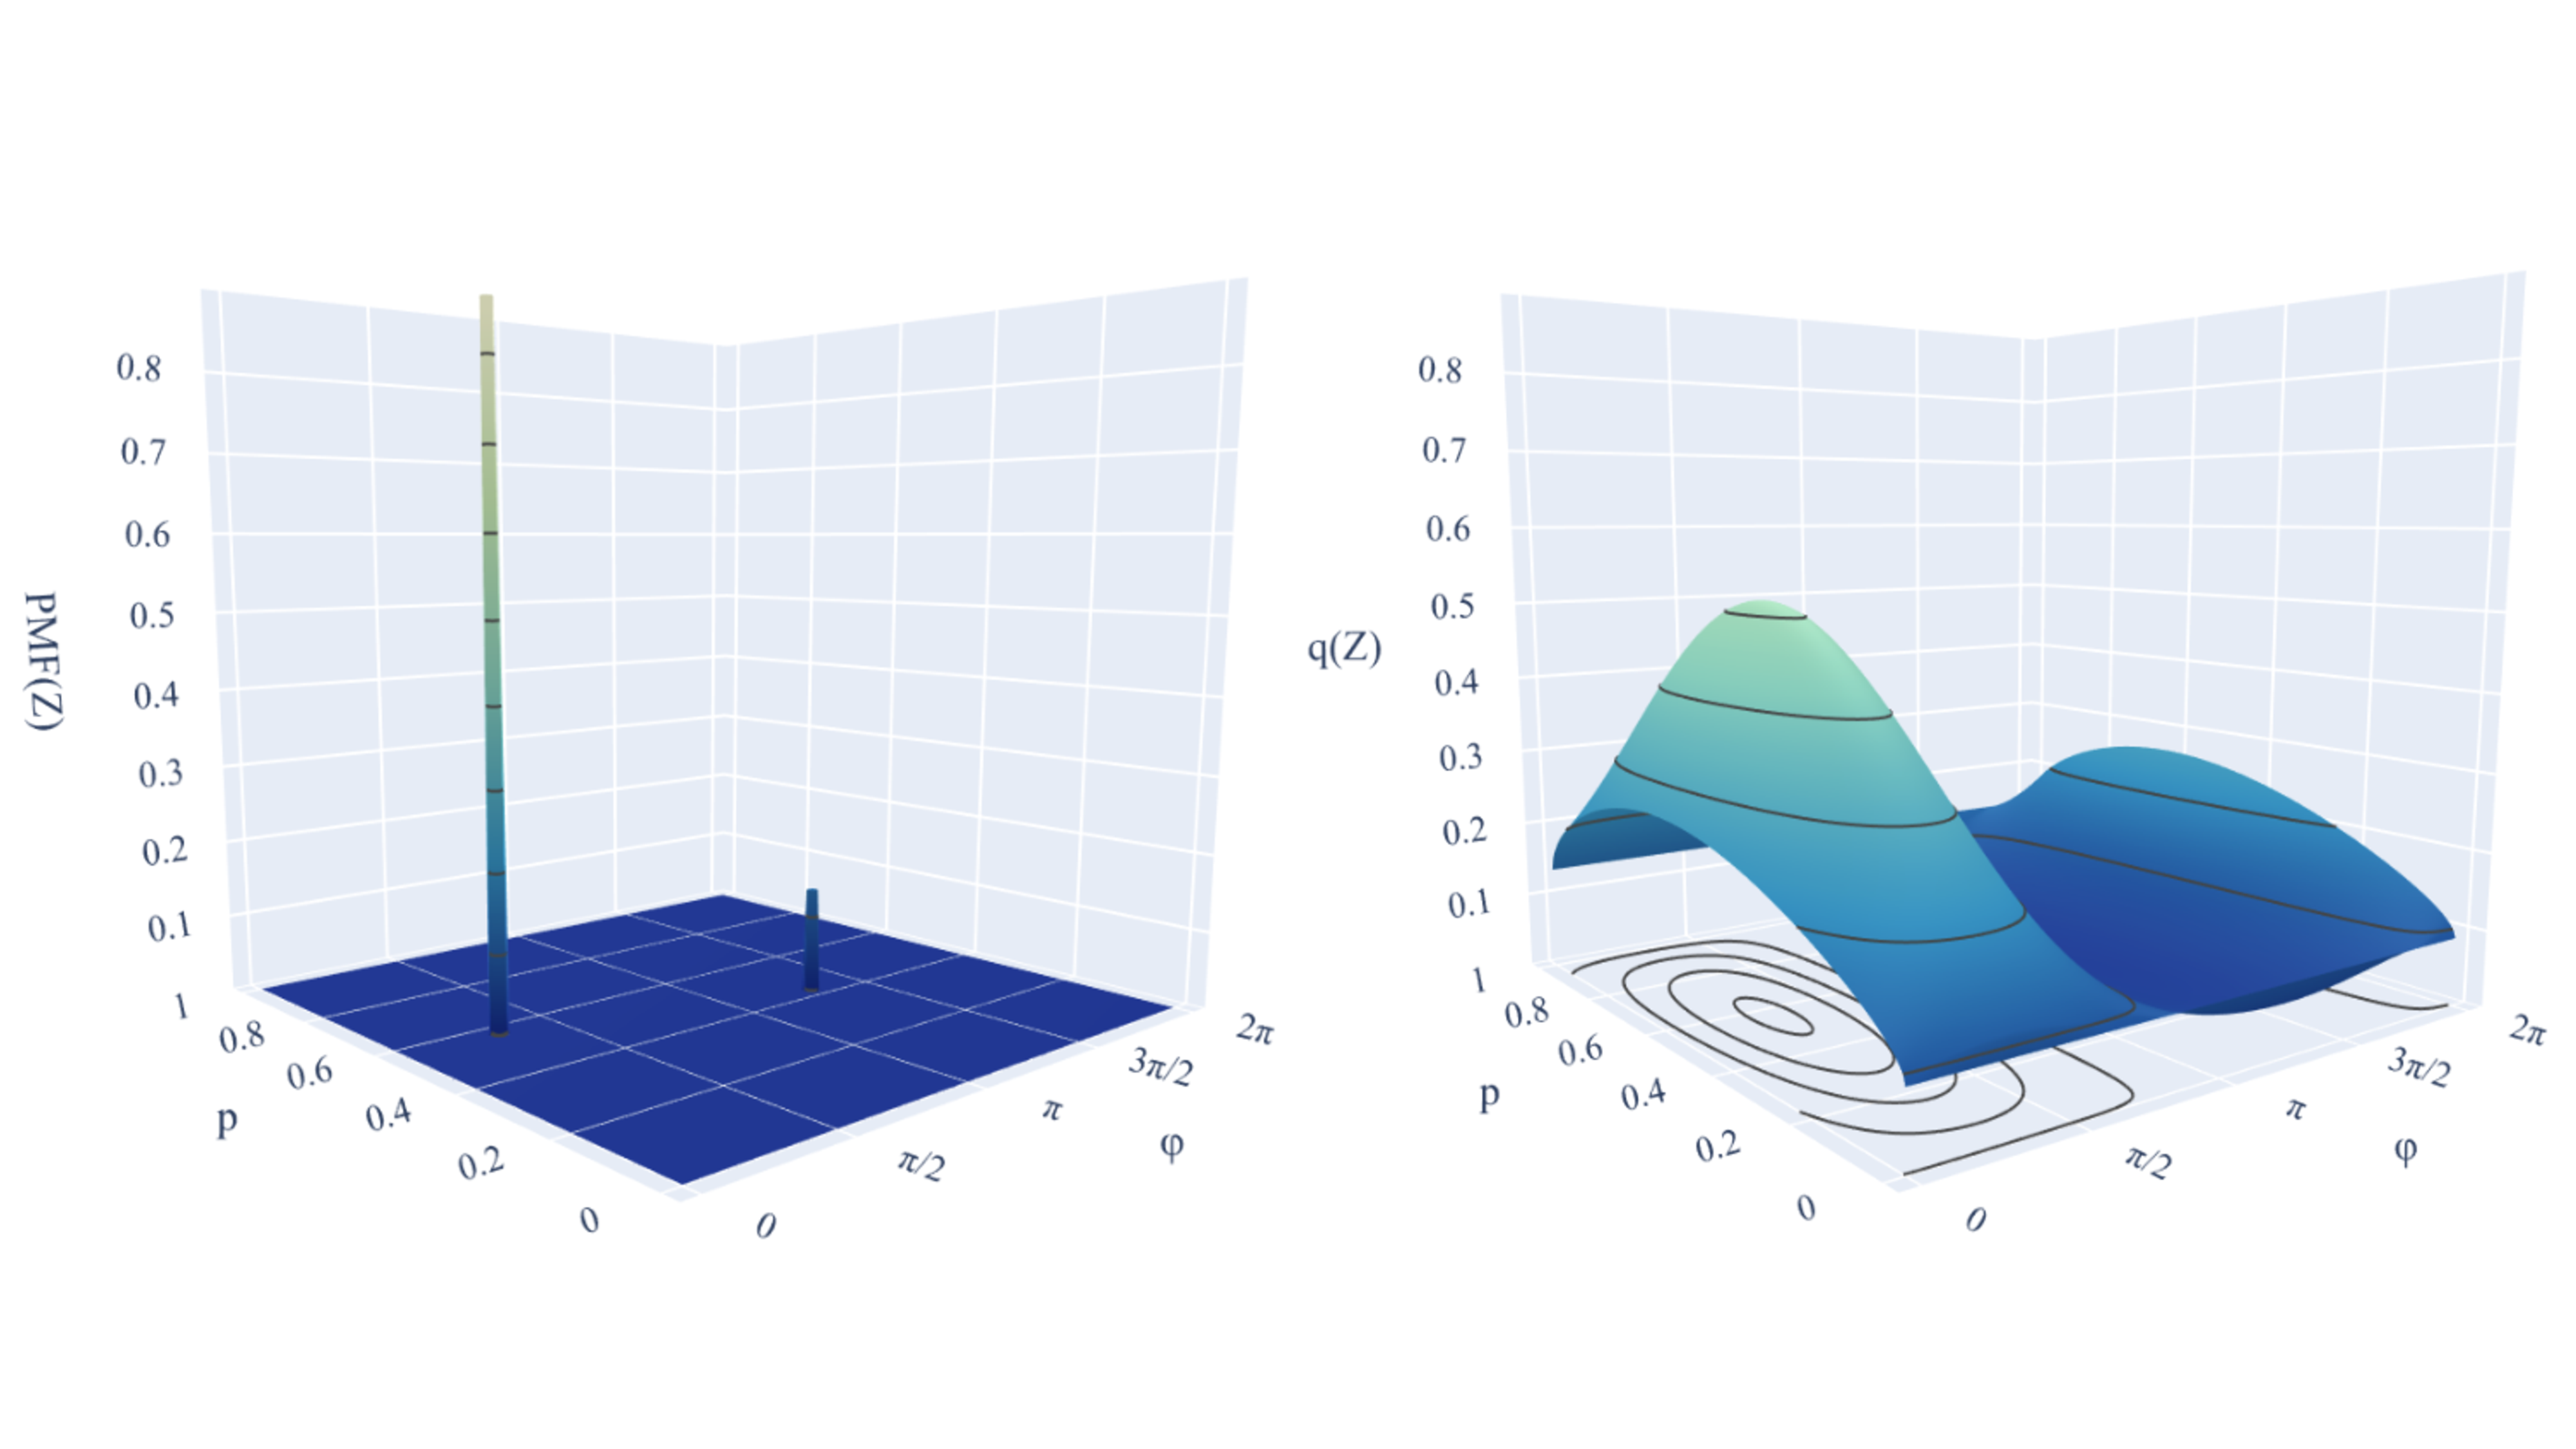
\includegraphics[width=\columnwidth]{img/New_Example.pdf}
\caption{Geometric quantum states in \emph{(probability,phase)} coordinates
	$(p,\phi)$ of $\mathbb{C}P^1$: (Left) Geometric quantum state $q_1$ is the
	convex sum of two Dirac delta-functions, centered on the eigenvectors
	$(p_+,\phi_+) = (0.568,0.983) $ and $(p_-, \phi_-) = (0.432,4.124)$ of
	density matrix $\rho$. (Right) Geometric quantum state $q_2$ differs
	markedly: A smooth distribution across the entire pure-state manifold
	$\mathbb{C}P^1$. However, $q_1$ and $q_2$ have the same density matrix
	$\rho_{q_1} = \rho_{q_2} = \rho$, where $\rho_{00} = 1- \rho_{11} = 0.45$,
	$\rho_{01} = \rho_{10}^{*} = 0.2 - 0.3 i$. $\rho_{\pm}$ are the eigenvalues
	of the density matrix: $\rho_+ = 0.864$ and $\rho_{-}=0.136$. Thus, the
	marked difference in the structure of geometric quantum states $q_1$ and
	$q_2$ is not reflected in their shared density-matrix $\rho_1 = \rho_2 =
	\rho$.
	}
\label{fig:Example} 
\end{figure}

This is particularly important for quantum information processing where one
encounters long-range and long-lived correlational and mechanistic demands.
Quantum computing immediately comes to mind. There, one is not only interested
in measurement outcomes, but also in predicting and understanding how a quantum
system evolves under repeated external manipulations imposed by complex control
protocols.

%In such settings, understanding whether a
%state-preparation protocol produces Dirac-delta-like distributions of pure
%states or more general distributions is paramount to properly address
%computational errors and to analyzing the thermodynamic costs of quantum
%computation.


\section*{Summary.}
Standard quantum mechanics' concept of state is the density matrix. However,
while density matrices provide a complete account of POVM statistics, they are
not in one-to-one correspondence with the ensembles that generated them. This
is a well-known fact that underlies the freedom in writing a decomposition of
the density matrix in terms of probabilities and pure states.  All such
decompositions yield the same POVM statistics, but they are not physically
equivalent since they are realized in physically different ways. The abiding
question then becomes: Which of these physically different ways exhibit
observable or, even perhaps, manipulable phenomena?

From a purification perspective \cite{Wilde2017}, the physical information
about an ensemble's realization can always be thought of as coming from a
larger system that is in a pure state. While the additional information about
how the ensemble is realized is not relevant for the measurement statistics on
our system, it does provide a much richer description. It preserves part (if
not all) of the structural information about how the system's POVM statistics
result from interactions with its surroundings.
 
Geometric quantum mechanics and its concept of geometric quantum state provide
a framework that allows retaining such information. This yields a richer
description of the system--one that goes beyond the system's POVM statistics, 
taking into account the physical manner in which an ensemble has been realized.
The geometric formalism's benefits emerge in at least two important cases:
(i) Hybrid continuous-discrete systems, e.g., electrons or other particles with
spin or other discrete degrees of freedom and (ii) the thermodynamic setting
of a system in contact with a large environment.

The geometric formalism directly handles the continuous nature of hybrid
systems and the large number of degrees of freedom in thermodynamics. And, it
does so in a fairly direct way. Thus, the geometric quantum state retains the 
structural information about how an ensemble is generated. While the 
two applications considered are similar, a crucial difference appears.

If we assume a finite environment, knowledge of the geometric quantum state of
our system is sufficient to recover the globally pure joint state of system and
environment. This does not occur for a hybrid discrete-continuous system, where
knowledge of the geometric quantum state does not allow inferring the phase
$\theta_0(\vec{x})$ of $f(\vec{x})$. Notably, fully recovering the overall pure
state, whose physical relevance can be argued on the ground of continuity with
the finite-dimensional case, effectively translates into a $U(1)$ gauge
principle on the overall system. The requirement that wave-functions differing 
from a local phase are physically equivalent---$\psi_s(\vec{x}) \sim
e^{i\varphi(\vec{x})}\psi_s(\vec{x})$---turns into a sufficient condition for
recovering the global pure state from the local geometric quantum state since, 
in this case, one can always choose $f(\vec{x}) \in \mathbb{R}$. Effectively, this is
the principle behind gauge symmetries and gauge theories. We must leave
exploring the connection between recovering the global pure state from a local
geometric quantum state and a gauge principle for a future investigation.

\paragraph*{Conclusion.}
Geometric quantum mechanics is an alternative to the standard vector-based
formalism. We introduced and then explored the concept of \emph{geometric
quantum state} $p(Z)$ as a probability distribution on the manifold of pure
states, inspired by the thermodynamic formalism of chaotic attractors from the
theory of dynamical systems or, more appropriately, its Sinai-Bowen-Ruelle
measures \cite{Eckmann1985}. This characterization accounts for the fact 
that singling out the density matrix as the sole descriptor of a quantum 
system's state entails ignoring how an ensemble is physically realized.
While this does not have observable consequences if one is restricted to POVM
statistics, in concrete situations the information about the ensemble
realization can be key to accurate modeling. Reference \cite{Anza20c} gives an
example. That said, the geometric setting is always sufficiently general
that density matrices are readily computed as quadratic averages from $p(Z)$
via Eq. (\ref{eq:densitymatrix}).

We explored the physical relevance of geometric quantum states via an open
quantum system in which a (finite) system under study is in contact with a
larger environment and their joint state is assumed to be pure. In this
thermodynamic setting, portions of the structural information about the joint
pure state is directly preserved in the geometric quantum state of the smaller
system under study. The result is a markedly richer picture of the system's
state---a picture that goes substantially beyond the density matrix and its
POVM statistics.

\section*{Acknowledgments}
\label{sec:acknowledgments}

F.A. thanks Marina Radulaski, Davide Pastorello, and Davide Girolami for
discussions on the geometric formalism of quantum mechanics. F.A. and J.P.C.
thank Dhurva Karkada for his help with the example and David Gier, Samuel
Loomis, and Ariadna Venegas-Li for helpful discussions and the Telluride
Science Research Center for its hospitality during visits.  This material is
based upon work supported by, or in part by, a Templeton World Charity
Foundation Power of Information Fellowship, FQXi Grant FQXi-RFP-IPW-1902, and
U.S. Army Research Laboratory and the U. S. Army Research Office under
contracts W911NF-13-1-0390 and W911NF-18-1-0028.

\bibliography{library}

\makeatletter
\newcommand{\manuallabel}[2]{\def\@currentlabel{#2}\label{#1}}
\makeatother

\clearpage
\appendix
\onecolumngrid

\pagestyle{empty}

\begin{center}
\large{Supplementary Materials}\\
\vspace{0.1in}
\emph{\ourTitle}\\
\vspace{0.1in}
{\small
Fabio Anza and James P. Crutchfield
}
\end{center}

\section{The Search for Quantum States}
\label{sm:QStates}

In those domains of the physical sciences that concern the organization and
evolution of systems, a common first task is to determine a system's distinct
configurations or \emph{effective states}. Ultimately, this turns on what
questions there are to answer. One goal is prediction---of properties or
behaviors. And, in this, quantum mechanics stands out as a particularly telling
arena in which to define effective states.

The very early history of its development can be construed partially as
attempts to answer this question, from de Broglie's \emph{phase-waves}
\cite{Brog25a} and Schrodinger's \emph{wave functions} \cite{Schr26a} to von
Neumann's \emph{statistical operators} in Refs. \cite{Neum27a} and \cite[Chap.
IV]{Neum32a}, later labeled \emph{density matrices} by Dirac
\cite{Dira29a,Dira30b,Dira31a}. And, these were paralleled by Heisenberg's
``operational'' \emph{matrix mechanics} that focused on experimentally
accessible observables and so avoided imputing internal, hidden structure
\cite{Heis25a}.

The abiding challenge is that effective states are almost always inferred
indirectly and through much trial and error. Quantum mechanics heightens the
challenge greatly due to its foundational axiom that the detailed, microscopic,
and fundamental degrees of freedom cannot be directly and completely measured
\emph{in principle}. The main text revisits this perennial question, What is a
quantum state?

\section{Theorem \ref{MainTheo}: Proof}
\label{sm:MainTheo}

This Appendix gives proves in detail Theorem \ref{MainTheo}.
Let's first restate its setup.

Consider a hybrid quantum system comprised of $N$ continuous degrees of freedom
and $M$ qudits that are the discrete ones. The entire system's Hilbert space
is:
\begin{align*}
\mathcal{H} = \mathcal{H}^c_N \otimes \mathcal{H}^d_M
  ~,
\end{align*}
where $\mathcal{H}_N^c$ hosts the continuous degrees of freedom and has
infinite dimension, while $\mathcal{H}^d_M$ hosts the discrete ones and has
dimension $d^M$. A basis for $\mathcal{H}_N^c$ is provided by
$\left\{\ket{\vec{x}}\right\}$, where $\vec{x} \in \mathcal{R} \subseteq
\mathbb{R}^N$ and a basis for $\mathcal{H}_M^d$ is
$\left\{\ket{s}\right\}_{s=0}^{d^M-1}$. Thus, a generic state is:
\begin{align}
\ket{\psi} = \int_{\mathcal{R}} d\vec{x} \sum_{s} \psi_s(\vec{x})\ket{\vec{x}} \ket{s}
  ~,\label{eq:first_step}
\end{align}
where $\vec{x}$ is a dimensionless counterpart of the physical continuous
degrees of freedom, achieved by multiplying its value by appropriate physical
quantities. So, the measure $d\vec{x}$ has no physical dimension. 


\emph{{\bf Theorem \ref{MainTheo}.}
Any state $\ket{\psi} \in \mathcal{H}$ can be written as:
\begin{align*}
\ket{\psi} = \int_{\mathcal{R}}d\vec{x} f(\vec{x}) \ket{x}\ket{q(\vec{x})}
  ~,
\end{align*}
where $f(\vec{x})$ is such that $\int_{\mathcal{R}}d\vec{x} |f(\vec{x})|^2 = 1$
and $\ket{q(\vec{x})}$ is a parametrized state of the discrete degrees of
freedom:
\begin{align*}
\ket{q(\vec{x})}
  = \sum_{s=0}^{d^M-1} \sqrt{p_s(\vec{x})} e^{i\phi_s(\vec{x})} \ket{s}
  ~,
\end{align*}
where $\left\{ p_s(\vec{x}),\phi_s(\vec{x})\right\}_s$ is a set of $2(d^M-1)$
real functions such that $\sum_{s=0}^{d^M-1} p_s(\vec{x}) = 1$,
$\phi_s(\vec{x}) \in [0,2\pi]$, and $\left\{\ket{s}\right\}_{s=0}^{d^M-1}$ is a
basis for $\mathcal{H}_M^d$.
}

\emph{Proof}: The proof is constructive. Given an arbitrary
$\left\{ \psi_s(\vec{x}) \right\}_s$, we can always find the set of functions
$f(\vec{x})$, $p_s(\vec{x})$, and $\phi_s(\vec{x})$. The converse holds
trivially: Given these functions one can always compute the $\left\{
\psi_s(\vec{x}) \right\}_s$. First, we define $\theta_s(\vec{x})$ as
the phase of $\psi_s(\vec{x})$:
\begin{align*}
\theta_s(\vec{x}) \in [0,2\pi[ \quad \mathrm{such \,\, that} \quad \psi_s(\vec{x}) = |\psi_s(\vec{x})| e^{i\theta_s(\vec{x})} 
  ~,
\end{align*}
and define the functions
\begin{align*}
\phi_s(\vec{x}) \coloneqq \theta_s(\vec{x}) - \theta_0(\vec{x})
  ~,
\end{align*}
Starting from Eq.(\ref{eq:first_step}) this gives

\begin{align*}
\ket{\psi} = \int_{\mathcal{R}} d\vec{x} \sum_{s} \psi_s(\vec{x})\ket{\vec{x}} \ket{s} = \int_{\mathcal{R}} d\vec{x} \sum_{s} \vert \psi_s(\vec{x}) \vert e^{i\theta_s(\vec{x})}\ket{\vec{x}} \ket{s} & =  \int_{\mathcal{R}} d\vec{x} \sum_{s} \vert \psi_s(\vec{x}) \vert e^{i\phi_s(\vec{x})+i\theta_0(\vec{x})}\ket{\vec{x}} \ket{s} \\ & = \int_{\mathcal{R}} d\vec{x} e^{i\theta_0(\vec{x})}\sum_{s} \vert \psi_s(\vec{x}) \vert e^{i\phi_s(\vec{x})}\ket{\vec{x}} \ket{s}
\end{align*}



We now define $f(\vec{x})$ and $p_s(\vec{x})$ as follows:
\begin{align*}
f(\vec{x}) & \coloneqq \sqrt{\sum_{s=0}^{d^M-1} \vert \psi_s(\vec{x}) \vert^2}
  \, e^{i \theta_0(\vec{x})} ~\text{and} \\
p_s(\vec{x}) & \coloneqq
  \frac{\vert \psi_s(\vec{x})\vert^2}{\sum_{l=0}^{d^M-1}\left\vert \psi_l(\vec{x})\right\vert^2}
  ~,
\end{align*}
It is easy to see how normalization of $|f(\vec{x})|^2$ and of $p_s(\vec{x})$ emerges from the definitions:
\begin{align*}
\int_{\mathcal{R}} d\vec{x} \left\vert f(\vec{x})\right\vert^2
  & = \int_{\mathcal{R}} d\vec{x}
  \sum_{s=0}^{d^M-1} \left\vert \psi_s(\vec{x}) \right\vert^2 \\
  & = 1 ~,\\
\sum_{s=0}^{d^M-1} p_s(\vec{x})
  & = \sum_{s=0}^{d^M-1}
  \frac{\vert \psi_s(\vec{x})\vert^2}{\sum_{l=0}^{d^M-1}\left\vert
  \psi_l(\vec{x})\right\vert^2} \\
  & = 1 ~,~\text{and} \\
\vert e^{i\phi_s(\vec{x})}\vert^2
  & = \frac{|\psi_s(\vec{s})|}{|\psi_s(\vec{x})|} \\
  & = 1
  ~.
\end{align*}
The latter gives $\phi_s(\vec{x}) \in [0,2\pi]$.

With these definitions we obtain:
\begin{align*}
e^{i\phi_s(\vec{x})} f(\vec{x}) \sqrt{p_s(\vec{x})}
  & = \sqrt{|\psi_s(\vec{x})|^2} e^{i\theta_s(\vec{x})} \\
  & = \psi_s(\vec{x})
  ~.
\end{align*}
This in turn gives the desired result:
\begin{align*}
\ket{\psi} & = \int_{\mathcal{R}} d\vec{x} \sum_{s} \psi_s(\vec{x})\ket{\vec{x}} \ket{s} \\
& = \int_{\mathcal{R}} d\vec{x} f(\vec{x}) \ket{\vec{x}}\sum_{s} e^{i\phi_s(\vec{x})}   \sqrt{p_s(\vec{x})}  \ket{s} \\
& = \int_{\mathcal{R}}d\vec{x} f(\vec{x}) \ket{x}\ket{q(\vec{x})}
  ~.
\end{align*}

%\bibliographystyleSM{apsr}
\bibliographySM{library}

\end{document}
